% !TeX root = ../main.tex
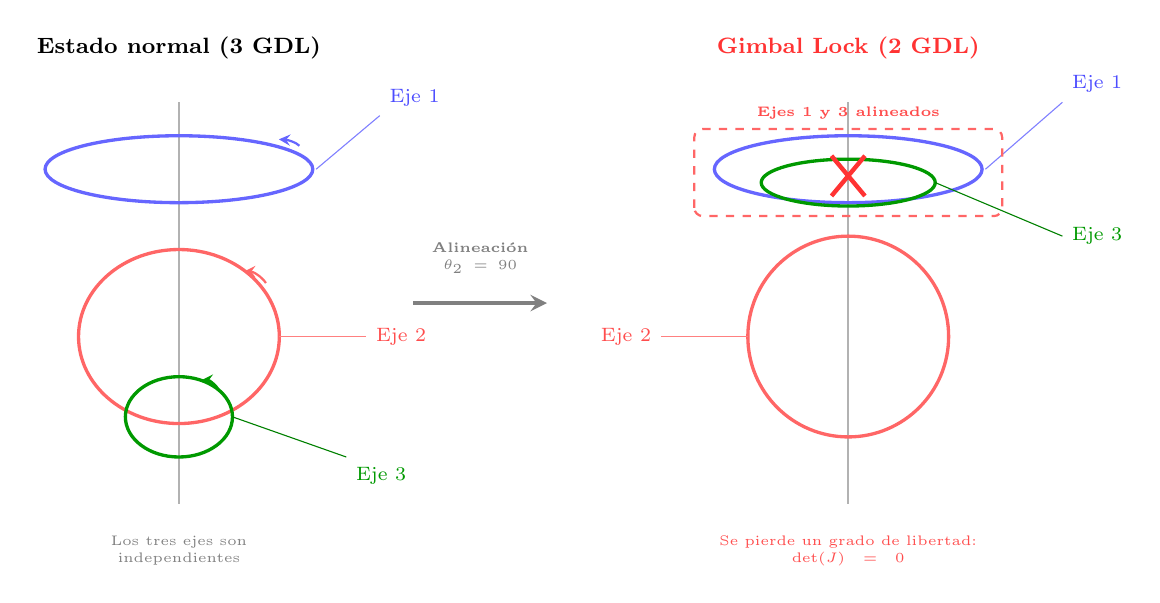
\begin{tikzpicture}[>=stealth, scale=0.85, every node/.style={font=\small}]

% =============================================
% PANEL IZQUIERDO: Estado Normal (3 GDL)
% =============================================
\begin{scope}[shift={(-5,0)}]
    \node[anchor=south, font=\bfseries\footnotesize] at (0, 4.0) {Estado normal (3 GDL)};
    
    % Eje vertical principal
    \draw[black!30, thick] (0,-2.5) -- (0,3.5);
    
    % Anillo exterior (Yaw) - arriba
    \draw[blue!60, very thick] (0,2.5) ellipse (2 and 0.5);
    \draw[->, blue!60, thick] (1.8,2.85) arc[start angle=20, end angle=80, x radius=0.4, y radius=0.15];
    % Etiqueta con línea guía hacia arriba
    \draw[blue!50, thin] (2.05,2.5) -- (3.0,3.3);
    \node[font=\scriptsize, blue!70, anchor=south west] at (3.0,3.3) {Eje 1};
    
    % Anillo medio (Pitch) - centro
    \draw[red!60, very thick] (0,0) ellipse (1.5 and 1.3);
    \draw[->, red!60, thick] (1.3,0.8) arc[start angle=35, end angle=90, radius=0.4];
    % Etiqueta con línea guía a la derecha
    \draw[red!50, thin] (1.5,0) -- (2.8,0);
    \node[font=\scriptsize, red!70, anchor=west] at (2.8,0) {Eje 2};
    
    % Anillo interior (Roll) - abajo
    \draw[green!60!black, very thick] (0,-1.2) ellipse (0.8 and 0.6);
    \draw[->, green!60!black, thick] (0.6,-0.8) arc[start angle=30, end angle=90, radius=0.3];
    % Etiqueta con línea guía abajo
    \draw[green!50!black, thin] (0.8,-1.2) -- (2.5,-1.8);
    \node[font=\scriptsize, green!60!black, anchor=north west] at (2.5,-1.8) {Eje 3};
    
    % Nota
    \node[font=\tiny, black!50, text width=3cm, align=center] at (0,-3.2) {Los tres ejes son\\independientes};
\end{scope}

% =============================================
% FLECHA CENTRAL
% =============================================
\draw[->, ultra thick, black!50] (-1.5,0.5) -- (0.5,0.5);
\node[anchor=south, font=\tiny\bfseries, black!50, text width=1.8cm, align=center] at (-0.5,0.8) {Alineación\\$\theta_2 = 90°$};

% =============================================
% PANEL DERECHO: Gimbal Lock (2 GDL)
% =============================================
\begin{scope}[shift={(5,0)}]
    \node[anchor=south, font=\bfseries\footnotesize, red!80] at (0, 4.0) {Gimbal Lock (2 GDL)};
    
    % Eje vertical principal
    \draw[black!30, thick] (0,-2.5) -- (0,3.5);
    
    % Anillo exterior (Yaw) — arriba
    \draw[blue!60, very thick] (0,2.5) ellipse (2 and 0.5);
    % Etiqueta Eje 1 — arriba a la derecha, bien separada
    \draw[blue!50, thin] (2.05,2.5) -- (3.2,3.5);
    \node[font=\scriptsize, blue!70, anchor=south west] at (3.2,3.5) {Eje 1};
    
    % Anillo interior ALINEADO con el exterior (¡el problema!)
    \draw[green!60!black, very thick] (0,2.3) ellipse (1.3 and 0.35);
    % Etiqueta Eje 3 — abajo a la derecha, separada del Eje 1
    \draw[green!50!black, thin] (1.3,2.3) -- (3.2,1.5);
    \node[font=\scriptsize, green!60!black, anchor=west] at (3.2,1.5) {Eje 3};
    
    % Anillo medio (Pitch) - girado 90° (ahora es un círculo grande)
    \draw[red!60, very thick] (0,0) ellipse (1.5 and 1.5);
    % Etiqueta Eje 2 — a la izquierda
    \draw[red!50, thin] (-1.5,0) -- (-2.8,0);
    \node[font=\scriptsize, red!70, anchor=east] at (-2.8,0) {Eje 2};
    
    % Cruz indicando GDL perdido (sobre la zona alineada)
    \draw[red!80, ultra thick] (-0.25,2.7) -- (0.25,2.1);
    \draw[red!80, ultra thick] (-0.25,2.1) -- (0.25,2.7);
    
    % Recuadro de alerta (solo alrededor de los ejes alineados)
    \draw[red!60, thick, dashed, rounded corners=3pt] (-2.3,1.8) rectangle (2.3,3.1);
    \node[font=\tiny\bfseries, red!70, anchor=south] at (0,3.1) {Ejes 1 y 3 alineados};
    
    % Nota
    \node[font=\tiny, red!70, text width=3.5cm, align=center] at (0,-3.2) {Se pierde un grado de libertad:\\$\det(J) = 0$};
\end{scope}

\end{tikzpicture}
